\section{Return Loss vs Frequency}

Another way of describing the efficiency of an antenna is with Return loss.
Return Loss is defined using the magnitude of the Reflection Coefficient $\Gamma$ in the following
form:
\begin{align}
  RL&=-20log|\Gamma|\text{dB}
\end{align}
In Figure~\ref{fig:rl}, it can be seen that as the frequency approaches 7MHz, the
value of the return loss reaches near -15dB. This is a desirable
(albeit non-ideal) value where little power is lost by returning to the
transceiver. 

\begin{figure}[h!]
  \centering
  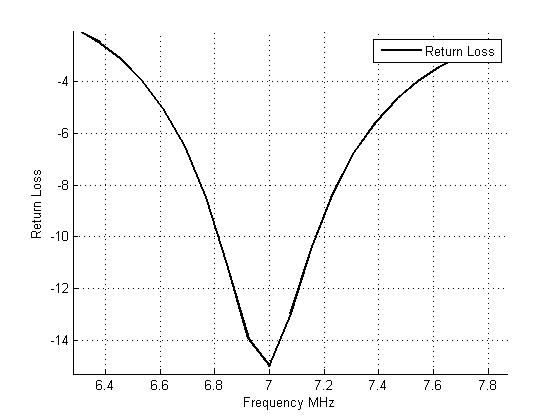
\includegraphics[width=0.45\textwidth]{./img/retloss.png}
  \caption{Return Loss versus Frequency}
  \label{fig:rl}
\end{figure}
